% ======== 学位論文 (ver1.1.1) ========= %
\RequirePackage{plautopatch}
\RequirePackage[l2tabu, orthodox]{nag}           % 古いものを一掃
\documentclass[platex, report, a4paper, 12pt, openany, twoside, dvipdfmx]{jlreq} % jlreqを用いる場合
% =======  プリアンブル ======== %
\usepackage{graphicx}                            % グラフ描画
\usepackage{xcolor}                              % 色の表示
\usepackage{amsmath, amssymb}                    % 数式全般
\usepackage{url}                                 % URL
\usepackage{multicol, multirow, booktabs}        % 表作成
\usepackage{hyperref}                            % ハイパーリンク
\usepackage{pxjahyper}                           % ↑(u)pLaTeXのときのみかく
\usepackage{titleps}                             % ノンブル・柱の変更
\usepackage[section]{placeins}                   % \section毎に図を調整
\usepackage[haranoaji]{pxchfon}                  % フォント指定([ms]: MS, [ipaex]: IPAexフォント)
\usepackage[deluxe]{otf}                         % 多書体化
\usepackage[margin=25truemm]{geometry}           % 余白設定(2023年度 Wordのテンプレートに準拠)
% \usepackage{cite}                                % (↓があるときはコメントアウト)参考文献をBibTeXでIEEEスタイルにする
\usepackage[%
  bibstyle=ieee,
  citestyle=numeric-comp,
  sorting=none,
  doi=false,
  eprint=false,
  url=true%
]{biblatex}                                      % (↑があるときはコメントアウト)参考文献をBibLaTeXでIEEEスタイルにする
% ======== bibLaTeXのファイルとオプション設定 ============ %
\addbibresource{references.bib} % bibファイルを拡張子つきで書く
% ======== ハイパーリンクの設定 by hyperref ========= %
\hypersetup{
  setpagesize=false,
  bookmarks=true,
  bookmarksnumbered=true,
  bookmarkstype=toc,
  colorlinks=true,
  urlcolor=black,
  linkcolor=black,
  citecolor=black
}
% ======== jlreqの各種設定 ========= %
% 図・表のキャプションの見た目変更
\jlreqsetup{
  caption_font=\normalsize,       % captionのフォント設定
  caption_label_font=\normalsize  % captionのラベルフォント設定
}
% ↓標準のスタイルの変更例
% \ModifyHeading{chapter}{font=\huge\gtfamily\bfseries}
% \ModifyHeading{section}{font=\Large\gtfamily\bfseries}
% \ModifyHeading{subsection}{font=\large\gtfamily\bfseries}
% \ModifyHeading{subsubsection}{font=\normalsize\gtfamily\bfseries}
% =======  ノンブル、柱の設定 ======== %
% == 目次での設定
% ヘッダーに全ての情報を載せる
\newpagestyle{headtypeTofCstyle}{
  \headrule
  \sethead[\scalebox{1.0}{\textbf{\thepage}}][][]
      {}{}{\scalebox{1.0}{\textbf{\thepage}}}
}
% == 本文での設定
% ヘッダーに全ての情報を載せる
\newpagestyle{headtypestyle}{
  \headrule
  \sethead[\scalebox{1.0}{\textbf{\thepage}}][][第\thechapter 章 \chaptertitle]
      {\thesection\quad\sectiontitle}{}{\scalebox{1.0}{\textbf{\thepage}}}
}
% == 参考文献・での設定
% ヘッダーに全ての情報を載せる
\newpagestyle{headtypestylePlain}{
  \headrule
  \sethead[\scalebox{1.0}{\textbf{\thepage}}][][\chaptertitle]
      {}{}{\scalebox{1.0}{\textbf{\thepage}}}
}
% == 付録での設定
% ヘッダーに全ての情報を載せる
\newpagestyle{headtypestyleAp}{
  \headrule
  \sethead[\scalebox{1.0}{\textbf{\thepage}}][][付録\thechapter \chaptertitle]
      {\thesection\quad\sectiontitle}{}{\scalebox{1.0}{\textbf{\thepage}}}
}
% =======  newcommandの使用例 ======== %
\newcommand{\img}{\mathrm{i}}         % 虚数単位
\newcommand{\e}{\mathrm{e}}           % Napier数
% =======  学位論文の報告者の情報 ======== %
% -- 学位の確認 -- %
\newcommand{\thesis}{修士論文}
\newcommand{\dept}{高知工科大学大学院工学研究科 \\ 基盤工学専攻○○○○工学コース}

% -- 報告者の情報 -- %
\renewcommand{\title}{タイトル(和文)}
\newcommand{\Etitle}{タイトル(英文)}
\newcommand{\studentID}{1XXXXXX}
\renewcommand{\author}{報告者の氏名}
\newcommand{\advisor}{指導教員の氏名と職階}
\renewcommand{\date}{\today}
% -- 表紙の空行による幅 [ \vskip -(2つのタイトルの行数-2)x20pt ] -- %
\newcommand{\adjspace}{\vskip -0pt}  % タイトルが複数行なら調節のために行間を減らす

% =======  表紙・本文のスタート ======== %
\begin{document}

% === 表紙 === %
% 表紙の設定です.
% 参考) TeXで表紙をカスタマイズして学位論文を書こう! Accessed on Nov.29, 2023, URL: https://satolog.org/tex-template/

\begin{titlepage}
  \fontsize{0.1cm}{0.1cm}\selectfont
  \textcolor{white}{empty} % 最初の改行を有効にするための補正

  \vskip 1.5cm  % 最初の改行, ??cm下げる \vskip ??cm

  \centering % 以降centering
  \fontsize{24pt}{0pt}\selectfont
  \textbf{\thesis}
    
  \vskip 1.6cm

  \fontsize{16pt}{20pt}\selectfont
  \title

  \vskip 0.5cm

  \fontsize{16pt}{20pt}\selectfont
  \Etitle

  % \vskip 4mm
  
  \rule[2mm]{14.7cm}{.2mm} % 横線を\rule[depth]{width}{height}で

  \vskip 3.2cm

  \adjspace % タイトルが複数行なら調節のために行間を減らす

  \fontsize{14pt}{15pt}\selectfont
  \textbf{報 告 者}
    
  \fontsize{12pt}{1.0cm}\selectfont
  学籍番号:\studentID
    
  \fontsize{12pt}{0.7cm}\selectfont
  氏名:\author

  \vskip -2mm
  \rule[0mm]{7cm}{.2mm}

  \vskip 1.5cm

  \fontsize{14pt}{14pt}\selectfont
  \textbf{指 導 教 員}

  \vskip 7mm

  \fontsize{12pt}{12pt}\selectfont
  \advisor

  \rule[0mm]{7cm}{.2mm}

  \vskip 1.9cm

  \fontsize{14pt}{0.9cm}\selectfont
  \date

  \vskip 1.9cm

  \fontsize{14pt}{20pt}\selectfont
  \textbf{\dept}
\end{titlepage}
\setcounter{page}{-1}%  初期値1

% === 目次 === %
\setcounter{page}{0}\pagenumbering{roman}\pagestyle{headtypeTofCstyle}
\tableofcontents
% \listoffigures
% \listoftables

% === 表目次のページ番号がローマ数字にならないバグの回避 === %
\newpage
\clearpage

% === 各種設定 === %
\graphicspath{{./figures/}} % グラフのあるパス
% main matterのノンブル・柱の設定
\setcounter{page}{0}\pagenumbering{arabic}
\pagestyle{headtypestyle}  % ヘッダーに全ての情報を載せる
% ========================= 本文開始 =================================== %

% == 本文
\chapter{main\_pLaTeX.texの設定}
基本的に\TeX Wiki~\cite{platex}や美文書作成入門~\cite{美文書作成入門},
main\_pLaTeX.texのコメントアウトを読めば分かるようにしているつもりである.
このテンプレートは2023年度高知工科大学 電子・光システム工学教室(以降,電子系と称する)の卒業論文・修士論文の要件を
満たすように作成したつもりだが、\textcolor{red}{今一度学位論文の要件を確認すること.}
作成者はこのテンプレートを用いることによる不利益に関しては保証しかねるのでご容赦を。。。
プリアンブルなどを調節したい場合は各自で行うこと.

このテンプレートは,ローカルではWindows10とWindows11のVisual Studio Codeで,
オンラインではOverleafとCloud LaTeXで動作実証済み($2023$年$12$月現在).
ただし,ローカルの場合は\TeX Live 2023で\LaTeX をインストールすることを前提としている.
\TeX Live以外にMac\TeX などがあるらしいが詳しいことは知らない.

\section{ここで使用する\LaTeX}
この \LaTeX はp\LaTeXe を採用している~\cite{美文書作成入門}.

\section{表紙の設定}
2023年度高知工科大学電子系の卒業論文・修士論文の表紙と一致するようにしたつもりだが,
今一度ご自身で印刷して確認すること.
一致していなければcover.tex内のファイルで表紙を制御しているので,
そのプログラムで調節すること.

記載する内容は卒業論文ならば\textbackslash newcommand\{\textbackslash thesis\}\{修士論文\}から
\textbackslash newcommand\{\textbackslash thesis\}\{学士論文\}のように変更すれば良い.
それ以外の箇所も同様である.変更する箇所は図\ref{fig:cover}の箇所である.

% === figure === %
\begin{figure}[h]
  \centering
  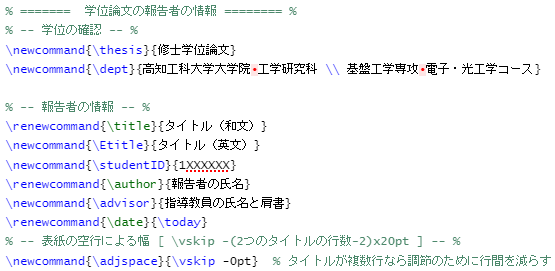
\includegraphics[keepaspectratio, width=0.75\linewidth]{verification_of_graduation.png}
  \caption{
    表紙の設定を記載する位置のスクリーンショット.main\_pLaTeX.texの$68$行目くらいにある.
    タイトルが合計で$2$行を超える場合は\textbackslash adjspace\{...\}で変更すること.}
  \label{fig:cover}
\end{figure}
% === figure === %

\section{ヘッダー・フッターの設定}
今設定しているヘッダー・フッターは,ヘッダーに下線を入れて小口にページ番号,のどに章・節を記載している.
変える箇所は図\ref{fig:nomble}にある.設定したヘッダー・フッターの出力結果は図\ref{fig:header}にある.

% === figure === %
\begin{figure}[h]
  \centering
  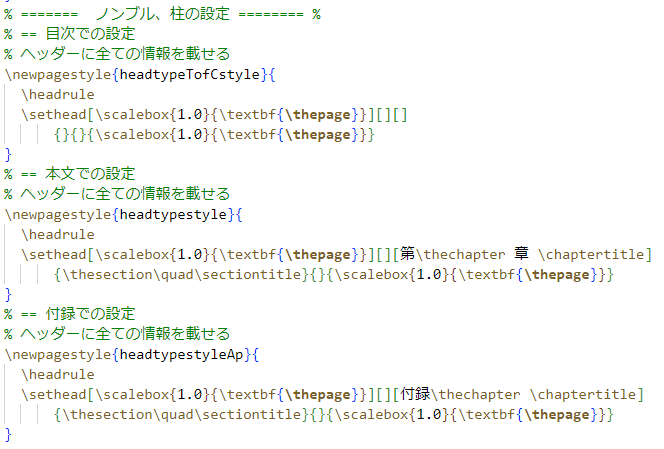
\includegraphics[keepaspectratio, width=0.9\linewidth]{nomble.png}
  \caption{ヘッダー・フッターの設定を記載した位置のスクリーンショット.main\_pLaTeX.texの$43$行目くらいにある.}
  \label{fig:nomble}
\end{figure}
% === figure === %
% === figure === %
\begin{figure}[h]
  \centering
  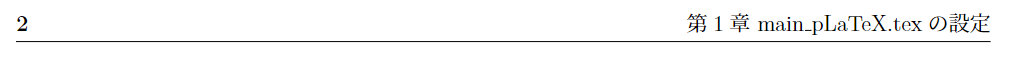
\includegraphics[keepaspectratio, width=0.9\linewidth]{header.png}
  \caption{ヘッダー・フッターの設定が反映された結果.}
  \label{fig:header}
\end{figure}
% === figure === %


\section{フォントの指定}
フォントに関しては,
\TeX Live 2020から標準和文の物理フォントの既定が
IPAexフォントから\textbf{\textsf{原ノ味フォント}}になったそう~\cite{font}.
変更方法は文献 \cite{font} が詳しい.
また,フロート~\cite{float}のキャプションがデフォルトで太字なので,
文献 \cite{jlreq} を参照して細字に変えた.
変更した箇所は図\ref{fig:jlreqset}にある.

% === figure === %
\begin{figure}[h]
  \centering
  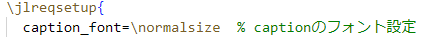
\includegraphics[keepaspectratio, width=0.75\linewidth]{jlreq_settings.png}
  \caption{フォントとjlreqの設定のスクリーンショット.main\_pLaTeX.texの$39$行目くらいにある.}
  \label{fig:jlreqset}
\end{figure}
% === figure === %


\section{目次の設定について}
目次と図目次,表目次は,main\_pLaTeX.texの91--93行目で制御している.
図目次と表目次を入れるかは各指導教官の方々の指示に従うようにすること.
$2023$年度の「卒業研究報告書(学士論文)・修士論文の執筆要項」では
図目次と表目次についての記載はないため,不要かもしれない.
使用する場合は \% でコメントアウトを外せば良い.

\subsection{表目次について}
表\ref{tab:triangle}に適当な表を作成した.
表目次を確認すると表\ref{tab:triangle}があることが分かる.

% === table === %
\begin{table}[htbp]
  \centering
  \caption{三角関数と双曲線関数}
  \begin{tabular}{cc} \hline 
    三角関数 & 双曲線関数 \\ \hline
    $\sin(x)$ & $\sinh(x)$ \\
    $\cos(x)$ & $\cosh(x)$ \\
    $\tan(x)$ & $\tanh(x)$ \\ \hline
  \end{tabular}
  \label{tab:triangle}
\end{table}
% === table === %


\subsection{図目次について}
図目次の動作は,図\ref{fig:cover}などを図目次と一致しているか確認すれば,
それぞれ対応する図ごとにページ番号が記載されていることが分かる.


\section{その他各種設定について}
上記の表紙やヘッダー・フッター,目次に加えて他にも,main\_LaTeX.tex内の
\textbackslash graphicspath\{\{./figures/\}\}の設定などがあるが,
細かい設定なのでここでは割愛する.

\chapter{参考文献について}
\section{引用順にソート済みであることの確認}
例えば,「$1935$年にA. Einsteinらは後に量子論が不完全と主張した~\cite{PhysRev.47.777}が,
彼らの主張では実験的に検証可能でなかった.
しかし,約$30$年の月日が経った$1964$年にJ. S. BellがA. Einsteinらの主張が検証可能であることを示した~\cite{PhysicsPhysiqueFizika.1.195}.」と書いて引用するとき,自動で引用順になる.

引用順になる理由は,
main\_LuaTeX.texでのbiblatexパッケージの公式ドキュメント~\cite{biblatex}を参照すること.

% === figure === %
\begin{figure}[h]
  \centering
  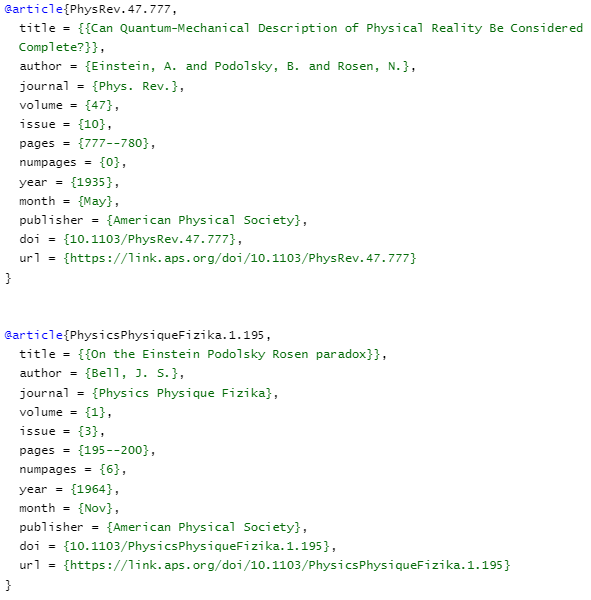
\includegraphics[keepaspectratio, width=0.6\linewidth]{ref_series.png}
  \caption{reference.bibの中にある参考文献の順番を表している図である.
  ``PhysicsPhysiqueFizika.1.195''が``PhysRev.47.777''よりも先に書かれているが,
  引用順は反対なため出力されたこのPDF内での参考文献の順番は反対になっている.
  したがって,参考文献をreferences.bibに載せる順番はまったく気にしなくてもよいことがいえる.}
  \label{fig:ref_series}
\end{figure}
% === figure === %

\section{参考文献の設定}
このテンプレートでは,Bib\LaTeX を採用した.
注意点としては,\textcolor{red}{Bib\TeX とは異なる}という点である.
このため,誤ってBib\TeX で検索しないように注意すること.
図\ref{fig:biblatex_settings}にBib\LaTeX の設定を示した.

このテンプレートでは,参考文献をIEEEスタイルで表示するようにしているが,
各指導教官の方々の指示に従い,変更点があるなら指示に従い変更すること.
なお,変更する際は公式ドキュメント~\cite{biblatex}やその他サイトで
検索して調べるように.

% === figure === %
\begin{figure}[h]
  \centering
  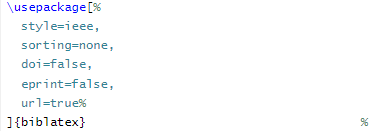
\includegraphics[keepaspectratio, width=0.6\linewidth]{biblatex_settings.png}
  \caption{main\_LuaTeX.texのBib\LaTeX の設定を示している.同ファイルの$16$行目にある.}
  \label{fig:biblatex_settings}
\end{figure}
% === figure === %

\section{Bibファイル編集の注意点}
図\ref{fig:ref_series}を見ると,titleを示す箇所が$2$重波括弧 \{\{\}\} で囲われている.
これは通常の波括弧 \{\} ではBib\LaTeX で先頭のみが大文字になる(有名な?)問題があり,
回避するには$2$重波括弧 \{\{\}\} で囲う必要があるそう.
Bibファイル内のtitleを自動で$2$重波括弧 \{\{\}\} にする方法は調べれば直ぐに出るが,
面倒なので作成していない.


% == 謝辞
\pagestyle{headtypestylePlain} % ノンブル・柱の設定
\addcontentsline{toc}{chapter}{謝辞}
\chapter*{謝辞}

指導教員や研究室のメンバーへの感謝などを書く.
特に,名前と職階は間違えないようにすること
(職階は高知工科大学のHPから直接コピー{\&}ペーストした方が確実.
名前も自分で打つよりコピー{\&}ペーストした方が間違えずに済む).


% == 参考文献
\pagestyle{headtypestylePlain} % ノンブル・柱の設定
\addcontentsline{toc}{chapter}{参考文献}
\printbibliography[title={参考文献}]  % 参考文献を表示 (biblatex)
% \bibliographystyle{jIEEEtran}  % 参考文献を表示 (bibtex, jIEEEtran.bstを使う場合)
% \bibliography{references}      % 参考文献を表示 (bibtex, .bibは省略)

% == ヘッダー・フッターのバグ回避
\newpage
\clearpage

% == 付録
\appendix  % 付録
\pagestyle{headtypestyleAp}  %ノンブル・柱の設定
\chapter{\LaTeX で図を用いるときのコツ} \label{apdx:tips}
PowerPointで図を作成してPNGやJPGなどで保存すると,デフォルトでは画像が粗くなる.
そこで,付録\ref{apdx:tips}ではPowerPointで作成した画像が
綺麗なまま\LaTeX で画像を表示させる方法を述べる.

以下,上記の手法の手順を示す.なお,以下のステップ$3$から$7$までの過程は図\ref{fig:method}に,
出力結果の例は\ref{fig:pdf}に示した.
\begin{enumerate}
    \item 予め,SVG画像を編集できるソフトをインストールし,使える状態にする
        (ここでは,Inkscapeというよく使われている無料ソフトを用いる~\cite{inkscape}).
    \item \LaTeX の編集ソフトとPowerPoint,Inkscapeの三つを開き,
        Inkscapeは新規ドキュメントを作成し待機する.
    \item PowerPointで保存したい図を選択し(グループ化しておくと確実),コピーする.
    \item コピーした画像を Inkscape の新規ドキュメントに貼り付ける.
    \item Inkscapeの「ファイル(F)」の「エクスポート(E)...」を選択(ショートカットキーはWindowsなら「Ctrl+Shift+E」).
    \item 右側にタブ(?)が現れ,「エクスポート(E)」のタブ上側の「ドキュメント」を選択し,
          画像サイズ(DPI)を上げる(作成者は$600$まで上げた).\\
          さらに,「エクスポート(E)」のタブ右下のフォーマットを変える箇所で「Portable Document Format(*.pdf)」を選択し,
          その左隣にあるフォルダアイコンをクリックする.
    \item 「エクスポートするファイル名」というポップアップが現れ,保存したいフォルダを選択した後,
          ファイル名を書いて保存する.
    \item 保存したPDFを確認すると,拡大しても画像が粗くないことが分かる.
    \item 画像を\LaTeX で参照すれば無事に図\ref{fig:pdf}のようになる.
    \item 次からの画像は,ステップ$3$から順に行なえば良い.
\end{enumerate}
ただし,ここで用いたInkspaceは$2023$年$12$月$1$日現在での最新版(Inkscape v.$1.3.2$)の場合であるため,
アップデートなどを経てUIが変わり分かりづらくなる可能性もある.

% === figure === %
\begin{figure}[h]
  \centering
  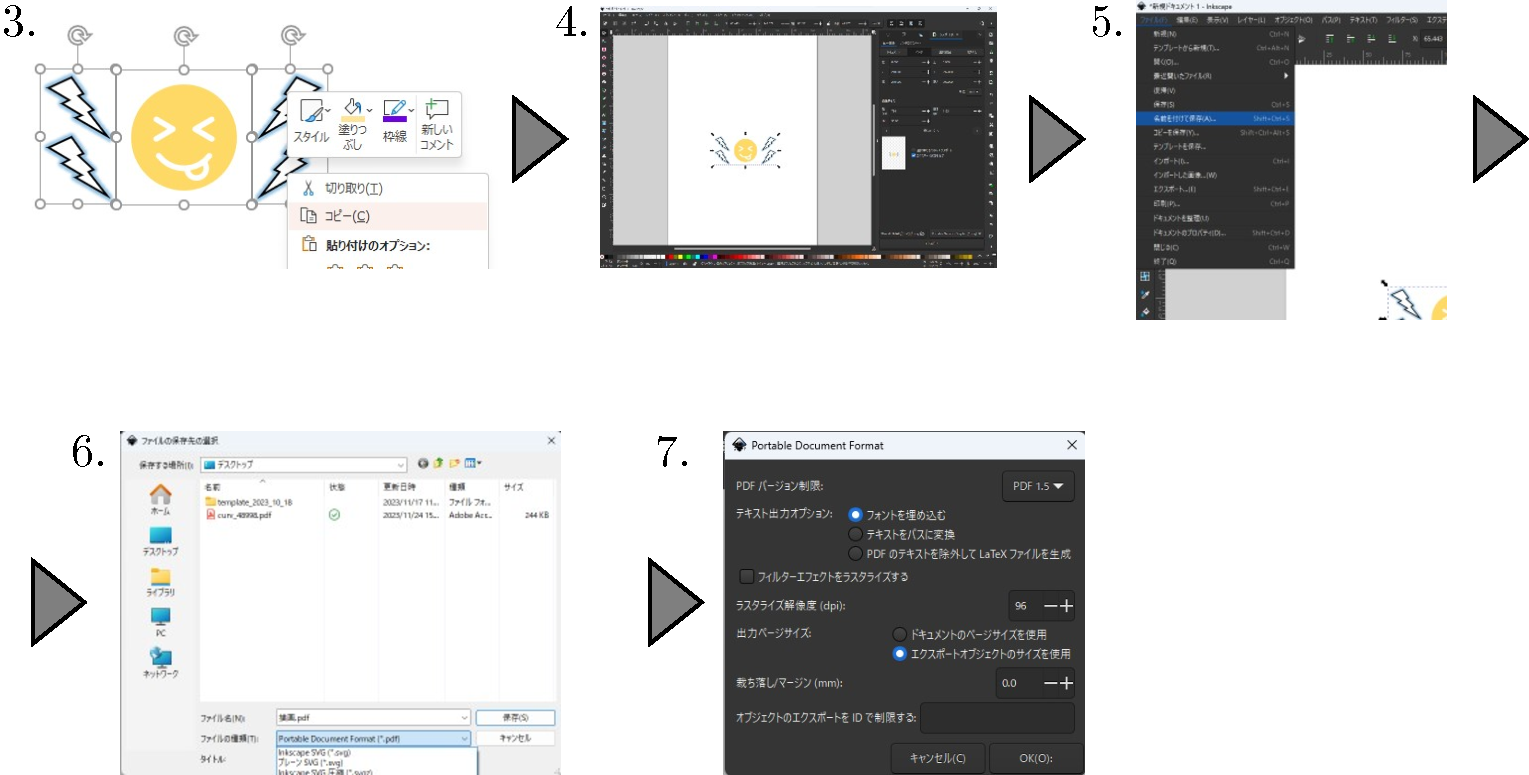
\includegraphics[keepaspectratio, width=0.9\linewidth]{method.png}
  \caption{ステップ$3$から$7$までの過程.
  スクリーンショットのため見づらいが拡大表示するなどして確認して欲しい.}
  \label{fig:method}
\end{figure}
% === figure === %
% === figure === %
\begin{figure}[h]
  \centering
  
\includegraphics[keepaspectratio, width=0.6\linewidth]{picture.pdf}
  \caption{作成したPDFファイル.拡大しても粗くならない.}
  \label{fig:pdf}
\end{figure}
% === figure === %

\chapter{日本語文献を用いる場合}
このテンプレートからも分かるように,日本語文献のタイトルは太字となってしまう.
これは,日本語の文献がBib{\LaTeX}側で考慮されていないことによるエラーである.
そこで,日本語でもIEEEスタイルで出力できるjIEEE.bstを使えば,タイトルが太字にならない.
しかし,標準ではjIEEEスタイルは\TeX Liveで同梱されていないのでダウンロードする必要がある~\cite{jieeetran}.
以下,jIEEEによる参考文献のスタイル変更の方法を記載する.

\begin{enumerate}
    \item jIEEEをGitHub~\cite{jieeetran}からダウンロードしてZIPファイルを解凍する.
    \item jIEEEtran-master/jIEEEtran にあるjIEEEtran.bstを作業フォルダ(main\_LuaTeX.texのあるフォルダ)に入れる.
    \item main\_LuaTeX.texで次の箇所を編集する.
        \begin{enumerate}
            \item \textbackslash usepackage[...]\{biblatex\} を \textbackslash usepackage\{cite\} に変更する.
            \item \textbackslash addbibresource\{references.bib\} を\% でコメントアウトする.
            \item \textbackslash printbibliography[title={参考文献}] を\% でコメントアウトする.
            \item 直前でコメントアウトした行の次の行で \textbackslash bibliography\{references\} と記述する.
            \item 更に,次の行で \textbackslash bibliographystyle\{jIEEEtran\} と記述する.
        \end{enumerate}
    \item 一度 \LaTeX ファイルをコンパイルする(まだ上手くいかない箇所があるはずだが).
    \item references.bib で次の箇所を編集する.
        \begin{enumerate}
            \item 作成したPDFで大文字が小文字で表示されたり,日本語の著者名が省略された場合,
                references.bib で該当箇所を$1$重波括弧\{\}から$2$重波括弧\{\{\}\}にする.\\
                (例. \{Accessed on Oct. 18, 2023\} を \{\{Accessed on Oct. 18, 2023\}\},\\
                    \{奥村晴彦, 黒木裕介\}を\{\{\{奥村晴彦, 黒木裕介\}\}\}に変更)
            \item 著書の一部を記載している場合,バッククォート二つとダブルクォート二つで書名を囲う.\\
                (例.[改定第$9$版]\LaTeXe 美文書作成入門が,``[改定第$9$版]\LaTeXe 美文書作成入門''となるはず)
        \end{enumerate}
\end{enumerate}

% ========================= 本文終了 =================================== %
\end{document}
